\chapter{Contribution}
The contributions produced by this project are:
\begin{itemize}
\item an \textbf{offloading system} conceived as a general architecture to be used in edge computing
\item a \textbf{path prediction system} that can be plugged into the offloading architecture and extended to different use cases
\end{itemize}

\section{Offloading System}
Edge computing is a recent computing paradigm that is trying to push data processing at the edge of the network, where the data is being generated. The goal is to reduce communication costs by keeping the computing close to the source of data. At the best of my knowledge, there hasn't been any effort in trying to implement a general abstraction - like the ISO/OSI stack (figure \ref{fig:iso_stack}) - which provides the guidelines for the protocol implementations. The proposed system is a first draft of how such abstraction could be implemented with all the limitations of a six-months work.
\begin{figure}[ht]
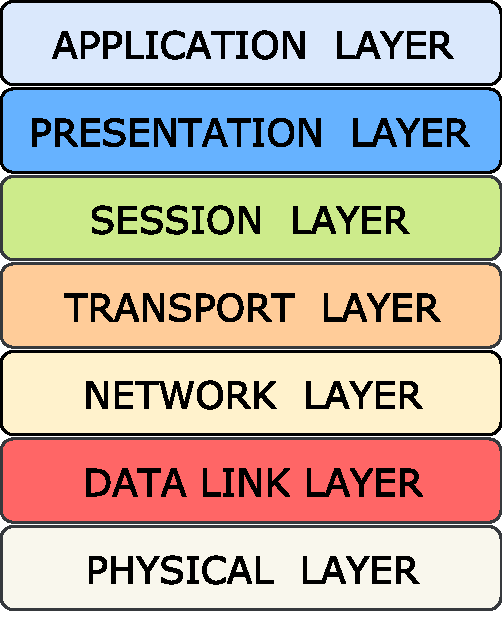
\includegraphics[width=\textwidth]{img/osi}
\caption{The ISO/OSI stack.}
\label{fig:iso_stack}
\end{figure}

\subsection{Architecture}
Before describing the architecture, it is necessary to list all the components involved in the edge computing scenario.
\subsection{Protocol}

\section{Path prediction System}
\subsection{Dataset}
\subsection{Model}